\documentclass[usenames,dvipsnames,aspectratio=169]{beamer}

%& PACKAGES
\usepackage[export]{adjustbox}
\usepackage{algorithm}
\usepackage{algorithmic}
\newcommand{\algorithmautorefname}{Algorithm}
%\usepackage[noend]{algorithmic}
%\usepackage[algo2e,vlined,ruled]{algorithm2e}
\usepackage{array}
\usepackage{amsmath,amsfonts,amssymb,amsthm}
%\usepackage[backend=bibtex,style=authoryear]{biblatex}
\usepackage{booktabs}
\usepackage{caption}
\usepackage{graphicx}
\usepackage{hyperref}
\usepackage[utf8x]{inputenc} % Xetex
\usepackage{mathtools}
\usepackage{multicol}
\usepackage{multirow}
\usepackage{pgfplots}
\usepackage{textpos}
\usepackage{tikz}
\usepackage{tikzsymbols}
\usepackage{xcolor}
\usetikzlibrary{shapes,fit,arrows,backgrounds,positioning,fadings,shadows,intersections, pgfplots.fillbetween,shapes.misc,automata}

%\usepackage{environ}
%\usepackage{breqn}
%\usepackage{tcolorbox}
%\usepackage{wasysym}
%\usepackage{transparent}
%\usepackage{relsize}
%\usepackage{appendixnumberbeamer}
%\usepackage[absolute,overlay]{textpos}
%\usepackage{setspace}
%\usepackage{makecell}
%\usepackage{wrapfig}

\hypersetup{
	colorlinks=false,
	urlcolor=cyan,
	citecolor=black
}


%& BEAMER SETTINGS
\usetheme{default}
\usecolortheme{seagull}
\setbeamertemplate{blocks}[rounded]% Rounded blocks
\setbeamertemplate{navigation symbols}{}
\setbeamertemplate{footline}[frame number]{} % frame number
%\setbeamertemplate{footline}{} % no frame number

%& BIB AND MACROS SOURCES
%\addbibresource{../icgp-bib.bib}
% Utils
% \newcommand{\todo}[1]{\textcolor{red}{\MakeUppercase{#1}}\\}
\newcommand{\tocite}[1]{ \textcolor{red}{[#1]} } 
\newcommand{\addlink}[2]{\href{#1}{#2}\footnote{\url{#1}}}
\def\code#1{\texttt{#1}}

\newcommand{\censor}[1]{#1}

% Standard algos
\newcommand{\neat}{NEAT}
\newcommand{\hyperneat}{HyperNEAT}
% \newcommand{\es}{evolution strategies}
\newcommand{\snes}{SNES}
\newcommand{\xnes}{XNES}
\newcommand{\enes}{eNES} 
\newcommand{\cmaes}{CMA-ES}
\newcommand{\sepcmaes}{sep-CMA-ES}
\newcommand{\openaies}{OpenAI ES}
\newcommand{\canonical}{Canonical ES}
\newcommand{\direct}{direct encoding}
\newcommand{\ars}{Augmented Random Search}


% My algos
%% GENE
% \newcommand{\gene}{GENE}
\newcommand{\coordsnet}{GENE}
\newcommand{\xdgene}{XD-GENE}
\newcommand{\ltwogene}{L2-GENE}
\newcommand{\grngene}{tag-GENE}
\newcommand{\pltwogene}{pL2-GENE}
\newcommand{\coordinates}{\textit{coordinates}}
\newcommand{\distfunc}{\textit{distance function}}

%% ES
% \newcommand{\dqnes}{DQNES}
\newcommand{\elitES}{ElitES}
% \newcommand{\mujoco}{\textsc{MuJoCo}}
\newcommand{\customes}{Custom ES}

\newcommand{\berl}{\code{BERL}}
\newcommand{\cambrian}{\code{Cambrian.jl} }

% Papers
\newcommand{\openaipaper}{\cite{salimansEvolutionStrategiesScalable2017}}
\newcommand{\canonicalpaper}{\cite{chrabaszczBackBasicsBenchmarking2018} }
\newcommand{\nespaper}{\cite{wierstraNaturalEvolutionStrategies2014}}
\newcommand{\aleguidelines}{\cite{machadoRevisitingArcadeLearning2017}}



%%% Text
\newcommand{\ie}{\emph{i.e.}}
\newcommand{\eg}{\emph{e.g.}}
\newcommand{\wrt}{\emph{w.r.t.}}
\newcommand{\etc}{\emph{e.t.c.}}
\newcommand{\onemax}{\textsc{OneMax}}
\newcommand{\leadingones}{\textsc{LeadingOnes}}
\newcommand{\procgen}{\textsc{ProcGen}}
\newcommand{\cartpole}{\textsc{CartPole}}
\newcommand{\acrobot}{\textsc{Acrobot}}
\newcommand{\pendulum}{\textsc{Pendulum}}
\newcommand{\mujoco}{\textsc{MuJoCo}}
\newcommand{\qm}[1]{``#1''}
% \newcommand{\note}[1]{{\color{blue}#1}}
\newcommand{\honemax}{H2}
\newcommand{\hleadingones}{H5}
\newcommand{\red}[1]{{\color{red}#1}}
% \newcommand{\lucie}{{\color{magenta}\texttt{LUCIE}}}

%%% Common Maths
\newcommand{\N}{\ensuremath{\mathbb{N}}}
\newcommand{\Z}{\ensuremath{\mathbb{Z}}}
\newcommand{\R}{\ensuremath{\mathbb{R}}}
\newcommand{\lnof}[1]{\ensuremath{\ln\left(#1\right)}}
\newcommand{\expof}[1]{\ensuremath{\exp\left(#1\right)}}
\newcommand{\powerof}[2]{\ensuremath{\left(#1\right)^{#2}}}
\newcommand{\set}[1]{\ensuremath{\left\{#1\right\}}}
\newcommand{\expect}{\ensuremath{\mathbb{E}}}
\newcommand{\expectof}[1]{\ensuremath{\expect{}\left(#1\right)}}
\newcommand{\proba}{\ensuremath{\mathbb{P}}}
\newcommand{\probaof}[1]{\ensuremath{\proba{}\left(#1\right)}}
\newcommand{\probaofgiven}[2]{\ensuremath{\proba{}\left(#1\;\middle|\;#2\right)}}
\newcommand{\union}[2]{\ensuremath{\bigcup\limits_{#1}^{#2}}}
\newcommand{\sumc}[2]{\ensuremath{\sum_{#1}^{#2}}} % condensed notation for sum
\newcommand{\intc}[2]{\ensuremath{\int_{#1}^{#2}}} % condensed notation for integral
\newcommand{\indic}[1]{\ensuremath{\boldsymbol{1}\left(#1\right)}} % indicatrice
%\newcommand{\intrange}[2]{\ensuremath{\left[#1,#2\right]}}
\newcommand{\intrange}[2]{\ensuremath{\left\{#1,\dots,#2\right\}}}
\newcommand{\eqdef}{\ensuremath{\stackrel{\text{def}}{=}}}
\newcommand{\bigo}{\ensuremath{\mathcal{O}}}
\newcommand{\bigoof}[1]{\ensuremath{\bigo{}\left(#1\right)}}
% \DeclarePairedDelimiter{\ceil}{\lceil}{\rceil}
% \DeclareMathOperator\erf{erf}
% \DeclareMathOperator*{\argmax}{arg\,max}
% \DeclareMathOperator*{\argmin}{arg\,min}

%%% Our Maths

% Constants
\newcommand{\csta}{\ensuremath{4}}
\newcommand{\cstatimestwo}{\ensuremath{8}}
\newcommand{\cstaminusone}{\ensuremath{3}}
\newcommand{\cstaminustwo}{\ensuremath{2}}
\newcommand{\cstb}{\ensuremath{2}}
\newcommand{\cst}[1]{\ensuremath{C_{#1}}}
\newcommand{\gammamax}{\ensuremath{0.57}}
\newcommand{\cstlemmathree}{\ensuremath{\tilde{C}}}
\newcommand{\npopmin}{\ensuremath{2}} % min total population size
\newcommand{\tmin}{\ensuremath{2}} % min number of steps
\newcommand{\deltamax}{\ensuremath{0.5}} % max value of delta

\newcommand{\npop}{\ensuremath{n}} % total population size
\newcommand{\nresampling}{\ensuremath{n_{\text{RS}}}}
\newcommand{\scalingfactor}{\ensuremath{\alpha}}
\newcommand{\nbits}{\ensuremath{N}} % Number of bits in OneMax and LeadingOnes
\newcommand{\budget}{\ensuremath{B}} % Max number of eval per generation for LUCBEA
\newcommand{\samplingstrategy}{\ensuremath{\mathcal{S}}}
\newcommand{\pbcomplexity}[2]{\ensuremath{H^{#1,#2}}}% pb complexity at gen #1 with factor #2
\newcommand{\meansymbol}[1]{\ensuremath{f}} % mean symbol
\newcommand{\mean}[1]{\ensuremath{\meansymbol{}_{#1}}}% mean of ind #1
\newcommand{\empiricalmean}[3]{\ensuremath{\hat{\meansymbol{}}_{#1}^{#2,#3}}}% empirical mean of ind #1 at gen #2 at time #3
\newcommand{\ttotal}{\ensuremath{N_{\text{non-term}}}}% total number of steps
\newcommand{\tremain}{\ensuremath{N_{\text{remain}}}}% number of remaining steps
\newcommand{\samplessymbol}{\ensuremath{u}}
%\newcommand{\samplesgensymbol}{\ensuremath{v}}
\newcommand{\nones}[1]{\ensuremath{D^{#1}}}% number of ones at generation #1
\newcommand{\opt}{\ensuremath{\text{opt}}}
\newcommand{\pes}{\ensuremath{\text{pes}}}
\newcommand{\xpesrv}[1]{\ensuremath{X^{\pes{}}_{#1}}}% rv X pessimal in leadingones with #1 leading ones
\newcommand{\xoptrv}[1]{\ensuremath{X^{\opt{}}_{#1}}}% rv X optimal in leadingones with #1 leading ones
\newcommand{\xpes}[1]{\ensuremath{x^{\pes{}}_{#1}}}% X pessimal in leadingones with #1 leading ones
\newcommand{\xopt}[1]{\ensuremath{x^{\opt{}}_{#1}}}% X optimal in leadingones with #1 leading ones
\newcommand{\observationsymbol}[1]{\ensuremath{O}}
\newcommand{\observationof}[1]{\ensuremath{\observationsymbol{}\left(#1\right)}}% observation of an ind #1 fitness
\newcommand{\nsamples}[3]{\ensuremath{\samplessymbol{}_{#1}^{#2,#3}}}% TOTAL number of samples of ind #1 at gen #2 at time #3
%\newcommand{\nsamplesgen}[3]{\ensuremath{\samplesgensymbol{}_{#1}^{#2,#3}}}% number of samples of ind #1 collected during gen #2 at step #3
\newcommand{\nsamplesstar}[3]{\ensuremath{\samplessymbol{}_{#1}^{*}(#3)}}% TOTAL number of samples of ind #1 at gen #2 at step #3 for bound to be lesser than max(delta_ind, epsilon/2)
%\newcommand{\nsamplesstargen}[3]{\ensuremath{\samplesgensymbol{}_{#1}^{*}(#2,#3)}}% number of samples of ind #1 collected during step #2 at time #3 for bound to be lesser than max(delta_ind, epsilon/2)
\newcommand{\nsamplesinit}[2]{\ensuremath{U_{#1}^{#2}}}% initial number of samples of ind #1 at gen #2
\newcommand{\nsamplesinitmax}[1]{\ensuremath{U^{#1}}}% max initial number of samples of gen #1
\newcommand{\boundsymbol}{\ensuremath{\beta}}
\newcommand{\bound}[3]{\ensuremath{\boundsymbol{}\left(#1,#3\right)}}% bound after #1 samples at step #3 of ind #2
\newcommand{\boundbarsymbol}{\ensuremath{\bar{\beta}}}
\newcommand{\boundbar}[3]{\ensuremath{\boundbarsymbol{}\left(#1,#3\right)}}% bound after #1 samples at step #3 of ind #2
\newcommand{\hucb}[2]{\ensuremath{h_{*}^{#1,#2}}} % highest UCB at gen #1 step #2
\newcommand{\llcb}[2]{\ensuremath{l_{*}^{#1,#2}}} % lowest LCB at gen #1 step #2
\newcommand{\hucbshort}[2]{\ensuremath{h^{#2}}}
\newcommand{\llcbshort}[2]{\ensuremath{l^{#2}}}
\newcommand{\maxc}[2]{\ensuremath{\left[#1\wedge#2\right]}} % condensed notation for max

% Sets
\newcommand{\individuals}[1]{\ensuremath{\textsc{Ind}^{#1}}} % Set of individuals of gen g
\newcommand{\topset}[1]{\ensuremath{\textsc{Top}^{#1}}} % top mu individuals of gen g
\newcommand{\botset}[1]{\ensuremath{\textsc{Bot}^{#1}}} % non-top mu individuals of gen g
\newcommand{\goodset}[1]{\ensuremath{\textsc{Good}^{#1}}} % epsilon-mu-optimal individuals of gen g
\newcommand{\badset}[1]{\ensuremath{\textsc{Bad}^{#1}}} % non-epsilon-mu-optimal individuals of gen g
\newcommand{\highset}[2]{\ensuremath{\textsc{High}^{#1,#2}}} % estimated top mu individuals at step t of gen g
\newcommand{\lowset}[2]{\ensuremath{\textsc{Low}^{#1,#2}}} % estimated non-top mu individuals at step t of gen g
\newcommand{\aboveset}[2]{\ensuremath{\textsc{Above}^{#1,#2}}} % middle at step t of gen g
\newcommand{\middleset}[2]{\ensuremath{\textsc{Middle}^{#1,#2}}} % middle at step t of gen g
\newcommand{\belowset}[2]{\ensuremath{\textsc{Below}^{#1,#2}}} % middle at step t of gen g

% Events
\newcommand{\failgen}[1]{\ensuremath{F^{#1}}}% fail gen #1
\newcommand{\failgenstep}[2]{\ensuremath{F^{#1}_{#2}}}% fail gen #1 step #2
\newcommand{\cross}[2]{\ensuremath{\textsc{Cross}^{#1,#2}}}
\newcommand{\crossind}[3]{\ensuremath{\textsc{Cross}_{#1}^{#2,#3}}}
\newcommand{\needy}[3]{\ensuremath{\textsc{Needy}_{#1}^{#2,#3}}}
\newcommand{\terminate}[2]{\ensuremath{\textsc{Term}^{#1,#2}}}


% My macros...
\newcommand*{\SET}[1]  {\ensuremath{\boldsymbol{#1}}}
\newcommand*{\VEC}[1]  {\ensuremath{\boldsymbol{#1}}}
\newcommand*{\MAT}[1]  {\ensuremath{\boldsymbol{#1}}}
\newcommand*{\OP}[1]  {\ensuremath{\text{#1}}}
\newcommand*{\NORM}[1]  {\ensuremath{\left\|#1\right\|}}
\newcommand*{\DPR}[2]  {\ensuremath{\left \langle #1,#2 \right \rangle}}
\newcommand*{\calbf}[1]  {\ensuremath{\boldsymbol{\mathcal{#1}}}}
\newcommand*{\shift}[1]  {\ensuremath{\boldsymbol{#1}}}
\newcommand{\argmax}{\operatornamewithlimits{argmax}}
\newcommand{\argmin}{\operatornamewithlimits{argmin}}
\newcommand{\ud}{\, \text{d}}
\newcommand{\vect}{\text{Vect}}
\newcommand{\sinc}{\text{sinc}}
\newcommand{\esp}{\ensuremath{\mathbb{E}}}
\newcommand{\hilbert}{\ensuremath{\mathcal{H}}}
\newcommand{\fourier}{\ensuremath{\mathcal{F}}}
\newcommand{\sgn}{\text{sgn}}
\newcommand{\intTT}{\int_{-T}^{T}}
\newcommand{\intT}{\int_{-\frac{T}{2}}^{\frac{T}{2}}}
\newcommand{\intinf}{\int_{-\infty}^{+\infty}}
\newcommand{\Sh}{\ensuremath{\boldsymbol{S}}}
\newcommand{\Cpx}{\ensuremath{\mathbb{C}}}
\newcommand{\K}{\ensuremath{\mathbb{K}}}
\newcommand{\reel}{\mathcal{R}}
\newcommand{\imag}{\mathcal{I}}
\newcommand{\cmnr}{c_{m,n}^\reel}
\newcommand{\cmni}{c_{m,n}^\imag}
\newcommand{\cnr}{c_{n}^\reel}
\newcommand{\cni}{c_{n}^\imag}
\newcommand{\LR}{\mathcal{L}_2(\R)}
\newcommand{\tproto}{g}
\newcommand{\rproto}{\check{g}}
\newcommand{\Tproto}{G}
\newcommand{\Rproto}{\check{G}}

%%% TIKZ

% fitness function
%\newcommand{\fit}[1]{{3+sin(54*#1-40)-0.2*#1}}
\newcommand{\fit}[1]{{2-0.1*#1+2.5*exp(-0.3*(#1-3)^2)+1.5*exp(-0.5*(#1-7)^2)}}

% plot a generation of indiv + their fitness
\newcommand{\plotgenf}[4]{% x color in-slide out-slide
\foreach \x in {#1}{%
	\onslide<#3-#4>{\node[ind,fill=#2] at (\x,0){};}
	\onslide<#4-#4>{\node[ind,fill=#2] at (\x,\fit{\x}){};}
}
}

% plot a generation of indiv + their fitness
\newcommand{\plotgen}[4]{% coord color in-slide out-slide
\foreach \x/\y in {#1}{%
	\onslide<#3-#4>{\node[ind,fill=#2] at (\x,0){};}
	\onslide<#4-#4>{\node[ind,fill=#2] at (\x,\y){};}
}
}

% plot a generation but only fitness
\newcommand{\plotgenonlyeval}[4]{% coord color in-slide out-slide
\foreach \x/\y in {#1}{%
	\onslide<#4-#4>{\node[ind,fill=#2] at (\x,\y){};}
}
}

% plot a one indiv and many eval
\newcommand{\plotgenmanyeval}[5]{% x ys color in-slide out-slide
	\onslide<#4-#5>{\node[ind,fill=#3] at (#1,0){};}
	\foreach \y in {#2}{%
		\onslide<#4-#5>{\node[ind,fill=#3] at (#1,\y){};}
	}
}

\newcommand{\squarebracket}[6]{% x y width color sidesize thickness
	\draw[color=#4, #6] (#1-#3,#2+#5) -- (#1-#3,#2) -- (#1+#3,#2) -- (#1+#3,#2+#5);
}

\newcommand{\roundbracket}[7]{% x y width color sidesize thickness rotate
	\begin{scope}[shift={(#1,#2)},rotate=#7]%
		\draw[color=#4,#6] (-#3+#5,0) -- (#3-#5,0);%
		\draw[color=#4,#6] (-#3,+#5) arc (0:90:-#5);%
		\draw[color=#4,#6] (#3,+#5) arc (0:-90:#5);%
	\end{scope}%
}

\def\bw{0.1} % confidence intervals width
\newcommand{\cifit}[4]{% x y beta color
	\draw[ultra thick, color=#4] (#1,#2-#3) -- (#1,#2+#3);
	\draw[ultra thick, color=#4] (#1-\bw,#2-#3) -- (#1+\bw,#2-#3);
	\draw[ultra thick, color=#4] (#1-\bw,#2+#3) -- (#1+\bw,#2+#3);
	\node[circle, draw=none, minimum width=0.2cm, inner sep=0, outer sep=0, fill=white, color=#4] at (#1,#2) {};
}

%& TITLES
\newcommand{\ti}{{$[$Context$]$}}
\newcommand{\tii}{{$[$Policy search$]$}}
\newcommand{\tiii}{{$[$Search space$]$}}
\newcommand{\tiv}{{$[$Search direction$]$}}
\newcommand{\tv}{{$[$Noisy fitness$]$}}
\newcommand{\tvi}{{$[$Directions$]$}}

\newcommand{\tei}{Context of this PhD}
\newcommand{\teii}{Evolution Strategies for Policy Search}
\newcommand{\teiii}{Representing policies and changing the search space}
\newcommand{\teiv}{Using samples to help the search}
\newcommand{\tev}{Adapting to stochastic problems}
\newcommand{\tevi}{Future work and timeline}

\newcommand{\tci}{{\color{teal} \ti{}}}
\newcommand{\tcii}{{\color{magenta} \tii{}}}
\newcommand{\tciii}{{\color{cyan} \tiii{}}}
\newcommand{\tciv}{{\color{ForestGreen} \tiv{}}}
\newcommand{\tcv}{{\color{orange} \tv{}}}
\newcommand{\tcvi}{{\color{Dandelion} \tvi{}}}

\newcommand{\es}{Evolution Strategies}
% \newcommand{\es}{\color{magenta} Evolution Strategies}
\newcommand{\gene}{GENE}
\newcommand{\dqnes}{DQNES}
% \newcommand{\dqnes}{\color{ForestGreen} DQNES}
\newcommand{\lucie}{\texttt{LUCIE}}
% \newcommand{\lucie}{\color{orange} \texttt{LUCIE}}
\newcommand{\fw}{Future Work}
% \newcommand{\fw}{\color{yellow} Future Work}



%& FONT
%\usefonttheme{serif}
%\setbeamerfont{normal text}{family=\rmfamily, size=\normalsize}
%\setbeamerfont{block body}{family=\rmfamily, size=\normalsize}
%\setbeamerfont{frametitle}{size=\Large} % default is \Large
\newcommand{\btVFill}{\vskip0pt plus 1filll}

%& multirows table cell
\newcommand{\cspecialcell}[2][c]{\begin{tabular}[#1]{@{}c@{}}#2\end{tabular}}
\newcommand{\lspecialcell}[2][l]{\begin{tabular}[#1]{@{}l@{}}#2\end{tabular}}

%& META-DATA
\title[Mid-thesis defense]{Evolution Strategies for Neural Policy Search}
\subtitle[]{Mid-thesis commitee}
\author{ 
	\textit{Author:} Paul Templier\textsuperscript{1} \\
	\textit{Advisors:} Emmanuel Rachelson\textsuperscript{1},
	Dennis G. Wilson\textsuperscript{1}\\
	\vspace{1em}
	\texttt{[paul.templier@isae-supaero.fr]}\\
	\vspace{1em}
	June 29, 2022\\
	\vspace{2em}
	\tiny \textsuperscript{1} University of Toulouse, ISAE-SUPAERO	
}
\date{June 29, 2022}

\begin{document}
\setbeamertemplate{caption}{\raggedright\insertcaption\par}
	
	\begin{frame}[plain,noframenumbering]{}%
		\begin{textblock*}{2cm}(-0.8cm,0cm) % {block width} (coords)
			\includegraphics[width=\textwidth]{images/misc/logo-isae-long.png}
		\end{textblock*}
		\vspace{2em}
		\titlepage
		\vspace{-6em}
	\end{frame}

	\begin{frame}{\tci{} Mid-thesis report}%

    \begin{center}
    %   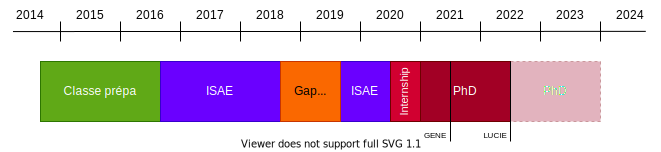
\includegraphics[width=12cm]{images/misc/timeline.drawio.png}

    \tikzset{every picture/.style={line width=0.75pt}} %set default line width to 0.75pt        

        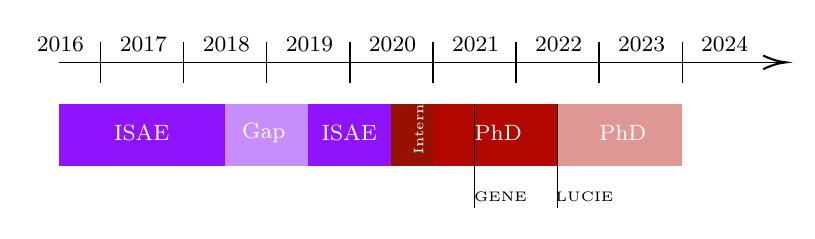
\begin{tikzpicture}[x=0.75pt,y=0.75pt,yscale=-1,xscale=1]
        %uncomment if require: \path (0,300); %set diagram left start at 0, and has height of 300

        %Axis 
        \draw    (80,110) -- (428,110) ;
        \draw [shift={(430,110)}, rotate = 180] [color={rgb, 255:red, 0; green, 0; blue, 0 }  ][line width=0.75]    (10.93,-3.29) .. controls (6.95,-1.4) and (3.31,-0.3) .. (0,0) .. controls (3.31,0.3) and (6.95,1.4) .. (10.93,3.29)   ;
        
        % Years 
        \draw (80.5,101.17) node  [font=\footnotesize] [align=left] {2016};
        \draw    (100,100) -- (100,120) ;
        \draw (120.5,101.17) node  [font=\footnotesize] [align=left] {2017};
        \draw    (140,100) -- (140,120) ;
        \draw (160.5,101.17) node  [font=\footnotesize] [align=left] {2018};
        \draw    (180,100) -- (180,120) ;
        \draw (200.5,101.17) node  [font=\footnotesize] [align=left] {2019};
        \draw    (220,100) -- (220,120) ;
        \draw (240.5,101.17) node  [font=\footnotesize] [align=left] {2020};
        \draw    (260,100) -- (260,120) ;
        \draw (280.5,101.17) node  [font=\footnotesize] [align=left] {2021};
        \draw    (300,100) -- (300,120) ;
        \draw (320.5,101.17) node  [font=\footnotesize] [align=left] {2022};
        \draw    (340,100) -- (340,120) ;
        \draw (360.5,101.17) node  [font=\footnotesize] [align=left] {2023};
        \draw    (380,100) -- (380,120) ;
        \draw (400.5,101.17) node  [font=\footnotesize] [align=left] {2024};
        
        % Blocks
        \draw  [draw opacity=0][fill={rgb, 255:red, 144; green, 19; blue, 254 }  ,fill opacity=1 ] (80,130) -- (160,130) -- (160,160) -- (80,160) -- cycle ;
        \draw  [draw opacity=0][fill={rgb, 255:red, 144; green, 19; blue, 254 }  ,fill opacity=1 ] (200,130) -- (240,130) -- (240,160) -- (200,160) -- cycle ;
        \draw  [draw opacity=0][fill={rgb, 255:red, 200; green, 141; blue, 252 }  ,fill opacity=1 ] (160,130) -- (200,130) -- (200,160) -- (160,160) -- cycle ;
        \draw  [draw opacity=0][fill={rgb, 255:red, 179; green, 8; blue, 0 }  ,fill opacity=1 ] (260,130) -- (320,130) -- (320,160) -- (260,160) -- cycle ;
        \draw  [draw opacity=0][fill={rgb, 255:red, 179; green, 8; blue, 0 }  ,fill opacity=0.42 ] (320,130) -- (380,130) -- (380,160) -- (320,160) -- cycle ;
        \draw  [draw opacity=0][fill={rgb, 255:red, 150; green, 17; blue, 0 }  ,fill opacity=1 ] (240,130) -- (260,130) -- (260,160) -- (240,160) -- cycle ;
        
        % Text
        \draw (120,144) node  [font=\footnotesize,color={rgb, 255:red, 255; green, 255; blue, 255 }  ,opacity=1 ] [align=left] {\begin{minipage}[lt]{20.4pt}\setlength\topsep{0pt}
        ISAE
        \end{minipage}};

        \draw (178.5,144) node  [font=\footnotesize,color={rgb, 255:red, 255; green, 255; blue, 255 }  ,opacity=1 ] [align=left] {\begin{minipage}[lt]{15.64pt}\setlength\topsep{0pt}
        Gap
        \end{minipage}};

        \draw (220,144) node  [font=\footnotesize,color={rgb, 255:red, 255; green, 255; blue, 255 }  ,opacity=1 ] [align=left] {\begin{minipage}[lt]{20.4pt}\setlength\topsep{0pt}
        ISAE
        \end{minipage}};
        
        \draw (253.09,148.63) node  [font=\tiny,color={rgb, 255:red, 255; green, 255; blue, 255 }  ,opacity=1 ,rotate=-270] [align=left] {\begin{minipage}[lt]{8.67pt}\setlength\topsep{0pt}
        Intern
        \end{minipage}};

        \draw (291,144) node  [font=\footnotesize,color={rgb, 255:red, 255; green, 255; blue, 255 }  ,opacity=1 ] [align=left] {\begin{minipage}[lt]{16.32pt}\setlength\topsep{0pt}
        PhD
        \end{minipage}};

        \draw (351,144) node  [font=\footnotesize,color={rgb, 255:red, 255; green, 255; blue, 255 }  ,opacity=1 ] [align=left] {\begin{minipage}[lt]{16.32pt}\setlength\topsep{0pt}
        PhD
        \end{minipage}};

    
        % Papers
        \draw    (280,130) -- (280,180) ;
        \draw (292.5,175) node  [font=\tiny] [align=left] {GENE};
        \draw    (320,130) -- (320,180) ;
        \draw (333,175) node  [font=\tiny] [align=left] {LUCIE};


    \end{tikzpicture}
    \end{center}

    \onslide<2->{
        \begin{block}{Initial topic}
          Bio-inspired methods for artificial neural networks
        \end{block}
      }

    \onslide<3->{
    \begin{block}{Goal of this report}
      Organize past and present work, and highlight future research directions.
    \end{block}
    }
\end{frame}

\begin{frame}{Content}
  \begin{enumerate}%
    \setlength\itemsep{1em}%
    \item<1-> \tci{} \tei{}
    \item<2-> \tcii{} \teii{}
    \item<3-> \tciii{} \teiii{}
    \item<4-> \tciv{} \teiv{}
    \item<5-> \tcv{} \tev{}
    \item<6-> \tcvi{} \tevi{}
  \end{enumerate}
\end{frame}


% \begin{frame}{\tci{} Goals of this defense}
%     \begin{itemize}%
%         \setlength\itemsep{1em}%
%         \item<2-> Present my work so far
%         \item<3-> Look at research directions 
%         \item<4-> Prioritize projects
%     \end{itemize}
% \end{frame}
	\begin{frame}{\tcii{} Policy search}
    \onslide<2->{
    \begin{center}
      \includegraphics[width=7cm]{images/misc/erl.png}\\
      \small \url{https://github.com/d9w/evolution/blob/master/imgs/erl.png}
    \end{center}
    }
\end{frame}

\begin{frame}{\tcii{} Neural networks}
    \begin{center}
      \includegraphics[width=8cm]{images/misc/dqn.png}\\
      \small Neural Network used in Deep Q Networks \cite{mnihHumanlevelControlDeep2015}
    \end{center}
\end{frame}

\begin{frame}{\tcii{} \es}
    \begin{center}
      \includegraphics[width=6cm]{images/misc/es.png}\\
      \small Evolution Strategy steps
    \end{center}
\end{frame}

\begin{frame}{\tcii{} Variants of \es}
    \onslide<1->{
    \begin{block}{Evolution Strategies}
        \begin{columns}
            \begin{column}{0.45\linewidth}
                \begin{itemize}
                    \item ($\mu , \lambda$) ES
                    \item \snes
                    \item Canonical ES 
                    \item OpenAI ES
                \end{itemize}
            \end{column}
            \begin{column}{0.45\linewidth}
                \begin{itemize}
                    \item \cmaes
                    \item \xnes
                    \item Cross-Entropy Method
                    \item Augmented Random Search
                \end{itemize}
            \end{column}
        \end{columns}
    \end{block}
    }
    \onslide<2->{   
    \begin{block}{Neuroevolution for policy search}
        \begin{itemize}
            \item large dimensions (1.6 $.10^6$ parameters)
            \item expensive evaluation 
        \end{itemize}
    \end{block}
    }
    
\end{frame}

\begin{frame}{\tcii{} \berl{}}

    \begin{block}{Reproduction settings}
        Reproducing \canonical{} \canonicalpaper{} and \openaies{} \openaipaper{} on the Arcade Learning Environment.
    \end{block}
    
    \begin{center}
        \begin{figure}
            \includegraphics[width=7cm]{images/BERL/Alien-v0.png}
            \caption{Evolution of \canonical{} and \openaies{} on Alien with 800 CPUh compute budget}
        \end{figure}
    \end{center}

\end{frame}
	% \include{slides/3-berl.tex}
	\begin{frame}{Content}
    \begin{enumerate}%
      \setlength\itemsep{1em}%
      \item {\color{lightgray} \ti{}} \tei{}
      \item {\color{lightgray} \tii{}} \teii{}
      \item {\color{lightgray} \tciii{}} \teiii{}
      \item {\color{lightgray} \tiv{}} \teiv{}
      \item {\color{lightgray} \tv{}} \tev{}
      \item {\color{lightgray} \tvi{}} \tevi{}
    \end{enumerate}
  \end{frame}

\begin{frame}{\tciii{} A Geometric Encoding for Neural Network Evolution}
    
    \begin{columns}
    \begin{column}{0.45\linewidth}
    \begin{center}
        \onslide<2->{
        \begin{figure}
        \centering
        \includegraphics[height=.7\linewidth]{images/GENE/images/gene_graph.png}
        \end{figure}
        }
    \end{center}
    \end{column}
    
    \begin{column}{0.45\linewidth}
    \begin{center}
        \onslide<3->{
        \begin{figure}
        \centering
        \includegraphics[height=.8\linewidth]{images/GENE/images/gene_coordinates.png}
        \end{figure}
        }
    \end{center}
    \end{column}
    \end{columns}
    
    \begin{columns}
    \begin{column}{0.45\linewidth}
    \begin{center}
        \onslide<2->{
        Fully connected \\ neural network
        }
    \end{center}
    \end{column}
    
    \begin{column}{0.45\linewidth}
    \begin{center}
        \onslide<3->{
            GENE encoding \\ {\color{lightgray} \cite{templierGeometricEncodingNeural2021}}
        }
    
    \end{center}
    \end{column}
    \end{columns}
    
\end{frame}


% L2 and signed
\begin{frame}{\tciii{} \gene: Distance functions}
    \begin{equation}
    w_{i, j} = dist(n_i, n_j)
    \end{equation}
    
    \begin{columns}
    \begin{column}{0.60\linewidth}
    \begin{block}{Euclidean distance}
    \begin{equation}
    \sqrt{\sum_{k=1}^D \left( n_1^k - n_2^k \right)^2 }
    \end{equation}
    \end{block}
    \end{column}
    
    \begin{column}{0.35\linewidth}
    \begin{figure}
    \centering
    \includegraphics[width=\linewidth]{images/GENE/images/distance_L2.png}
    \end{figure}
    \end{column}
    \end{columns}
    
    % \begin{block}{Euclidean distance}
    
    % \end{equation}
    % \end{block}
    
\end{frame}

% Weights
\begin{frame}{\tciii{} \gene: Weight distribution}
    
    \begin{figure}
    \centering
    \includegraphics[width=.7\linewidth]{images/GENE/images/weights_distrib.png}
\end{figure}
\begin{center}
    \small Distribution of weight values in networks evolved with different encodings.
\end{center}
\end{frame}

\begin{frame}{\tciii{} Experimental setup}
\begin{columns}
        
    \begin{column}{0.7\linewidth}
    \begin{center}
        \begin{figure}
        \centering
        \includegraphics[width=.7\linewidth]{images/GENE/images/RAM_net.png}
        \small \\ RAM state representation
          \end{figure}
    
    \end{center}
    \end{column}
    
    \begin{column}{0.3\linewidth}
    \begin{center}
    \onslide<2->{
        \begin{block}{SNES}
            \begin{itemize}
                \item Separable NES 
                \item Complexity in $O(n)$
            \end{itemize}
        \end{block}

        \begin{block}{XNES}  
            \begin{itemize}
                \item Exponential NES
                \item Complexity in $O(n^2)$
            \end{itemize}
        \end{block}
    }
    \onslide<3->{
        \begin{block}{Encodings}  
            \begin{itemize}
                \item Direct encoding
                \item GENE: dim=3
                \item 10 runs
            \end{itemize}
        \end{block}
    }
    \end{center}
    \end{column}

    \end{columns}
\end{frame}


% Update step
\begin{frame}{\tciii{} Computational cost}
    
    \begin{block}{Evolutionary Strategy update of $\mu$ and $\sigma$} 
            \begin{table}
                \begin{tabular}{llllrr}
                        Encoding  & $D$ & Genes &  &  Mean time (s) &  Memory (KiB) \\
                    \midrule
                    \pltwogene{} &   3 & 804 & SNES &       0.000357 &                 630.56 \\
                    \pltwogene{} &  10 & 2211 & SNES &       0.000678 &                1372.16 \\
                     Direct &   - & 5609 & SNES &       0.001350 &                3133.44 \\
                    \pltwogene{} &   3 & 804 & XNES &       1.475000 &             1352663.04 \\
                    \pltwogene{} &  10 & 2211 & XNES &      14.244000 &            11806965.76 \\
                     Direct &   - & 5609 & XNES &     119.976000 &            79765176.32 \\
                    \end{tabular}
    %            \caption{Average time and memory for the build step of 1 individual, for a 128-32-32-9 network. All \coordsnet{} functions have similar build time, so only \pltwogene{} is used.}
            \end{table}
        \end{block}
    \end{frame}


% Results
\begin{frame}{\tciii{} Competitive results - Arcade Learning Environment}
    \onslide<1->{
    %SpaceInvaders
    \begin{columns}
      \begin{column}{0.45\linewidth}
        \begin{center}
          \begin{figure}
              \centering
              \includegraphics[width=.9\linewidth]{images/GENE/plots/SpaceInvaders - 128-64-64-6 - snes.png}
        \small SNES on SpaceInvaders
          \end{figure}
        \end{center}
      \end{column}
      
      \begin{column}{0.45\linewidth}
        \begin{center}
          \begin{figure}
              \centering
   \includegraphics[width=.9\linewidth]{images/GENE/plots/SpaceInvaders - 128-64-64-6 - xnes.png}
        \small XNES on SpaceInvaders
          \end{figure}
        \end{center}
      \end{column}
    \end{columns}
    }

    \onslide<2->{
    % Seaquest
     \begin{columns}
      \begin{column}{0.45\linewidth}
        \begin{center}
          \begin{figure}
              \centering
              \includegraphics[width=.9\linewidth]{images/GENE/plots/krull - 128-64-64-18 - snes.png}
        \small SNES on Krull
          \end{figure}
        \end{center}
      \end{column}
      
      \begin{column}{0.45\linewidth}
        \begin{center}
          \begin{figure}
              \centering
   \includegraphics[width=.9\linewidth]{images/GENE/plots/krull - 128-64-64-18 - xnes.png}
        \small XNES on Krull
          \end{figure}
        \end{center}
      \end{column}
    \end{columns}
    }
  
  \end{frame}
  
  % Results
  \begin{frame}{\tciii{} Improving results - Arcade Learning Environment}
    \onslide<1->{
    %IceHockey
    \begin{columns}
      \begin{column}{0.45\linewidth}
        \begin{center}
          \begin{figure}
              \centering
              \includegraphics[width=.9\linewidth]{images/GENE/plots/IceHockey - 128-64-64-18 - snes.png}
        \small SNES on IceHockey
          \end{figure}
        \end{center}
      \end{column}
      
      \begin{column}{0.45\linewidth}
        \begin{center}
          \begin{figure}
              \centering
   \includegraphics[width=.9\linewidth]{images/GENE/plots/IceHockey - 128-64-64-18 - xnes.png}
        \small XNES on IceHockey
          \end{figure}
        \end{center}
      \end{column}
    \end{columns}
    }
    \onslide<2->{
    % Seaquest
     \begin{columns}
      \begin{column}{0.45\linewidth}
        \begin{center}
          \begin{figure}
              \centering
              \includegraphics[width=.9\linewidth]{images/GENE/plots/seaquest - 128-64-64-18 - snes.png}
        \small SNES on Seaquest
          \end{figure}
        \end{center}
      \end{column}
      
      \begin{column}{0.45\linewidth}
        \begin{center}
          \begin{figure}
              \centering
   \includegraphics[width=.9\linewidth]{images/GENE/plots/seaquest - 128-64-64-18 - xnes.png}
        \small XNES on Seaquest
          \end{figure}
        \end{center}
      \end{column}
    \end{columns}
    }
  \end{frame}
  
  
  \begin{frame}{\tciii{} \fw}
    
    \begin{columns}
    \begin{column}{0.45\linewidth}
    \begin{center}
    \begin{block}{Distance functions}
    Design new distance functions, or optimize them through co-evolution.
    \end{block}
    
    \begin{block}{Hybrid encoding}
    Switch between indirect and direct encodings during the evolution.
    \end{block}
    \end{center}
    \end{column}
    
    \begin{column}{0.45\linewidth}
    \begin{center}
    \begin{block}{Gradient descent}
    Use backpropagation and gradient descent to optimize genomes instead of evolution.
    \end{block}
    
    \begin{block}{Complex networks}
    Design encodings for convolution layers and recurrent networks.
    \end{block}
    \end{center}
    \end{column}
    \end{columns}
    
    \end{frame}
	% \begin{frame}{\tciv{} \dqnes{}}
%     \onslide<2->{
%     \begin{figure}
%     \centering
%     \includegraphics[width=.7\linewidth]{images/DQNES/scheduled.drawio.png}
%     \caption{Distribution of weight values in networks evolved with different encodings.}
%     \end{figure}
%     }
% \end{frame}

\begin{frame}{\tciv{} Using samples to drive the search}%
    \begin{figure}


    \tikzset{every picture/.style={line width=0.75pt}} %set default line width to 0.75pt        

    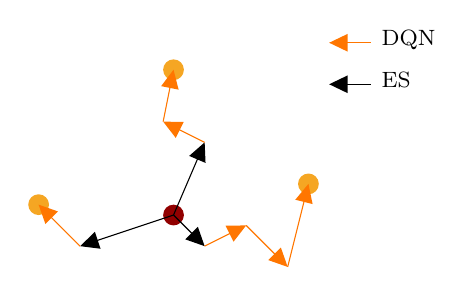
\begin{tikzpicture}[x=0.75pt,y=0.75pt,yscale=-1,xscale=1]
    %uncomment if require: \path (0,300); %set diagram left start at 0, and has height of 300
        % Center
        \onslide<2->{
        %Flowchart: Connector [id:dp7892172092869572] 
        \draw  [draw opacity=0][fill={rgb, 255:red, 145; green, 0; blue, 0 }  ,fill opacity=1 ] (270,155) .. controls (270,152.24) and (272.24,150) .. (275,150) .. controls (277.76,150) and (280,152.24) .. (280,155) .. controls (280,157.76) and (277.76,160) .. (275,160) .. controls (272.24,160) and (270,157.76) .. (270,155) -- cycle ;
        }

        % End points
        \onslide<4->{
        %Flowchart: Connector [id:dp8059049646076628] 
        \draw  [draw opacity=0][fill={rgb, 255:red, 245; green, 166; blue, 35 }  ,fill opacity=1 ] (205,150) .. controls (205,147.24) and (207.24,145) .. (210,145) .. controls (212.76,145) and (215,147.24) .. (215,150) .. controls (215,152.76) and (212.76,155) .. (210,155) .. controls (207.24,155) and (205,152.76) .. (205,150) -- cycle ;
        %Flowchart: Connector [id:dp5011381675096028] 
        \draw  [draw opacity=0][fill={rgb, 255:red, 245; green, 166; blue, 35 }  ,fill opacity=1 ] (270,85) .. controls (270,82.24) and (272.24,80) .. (275,80) .. controls (277.76,80) and (280,82.24) .. (280,85) .. controls (280,87.76) and (277.76,90) .. (275,90) .. controls (272.24,90) and (270,87.76) .. (270,85) -- cycle ;
        %Flowchart: Connector [id:dp3773909027910184] 
        \draw  [draw opacity=0][fill={rgb, 255:red, 245; green, 166; blue, 35 }  ,fill opacity=1 ] (335,140) .. controls (335,137.24) and (337.24,135) .. (340,135) .. controls (342.76,135) and (345,137.24) .. (345,140) .. controls (345,142.76) and (342.76,145) .. (340,145) .. controls (337.24,145) and (335,142.76) .. (335,140) -- cycle ;
        }

        \onslide<3->{
        %Straight Lines [id:da6809885341795275] 
        \draw    (275,155) -- (232.85,169.05) ;
        \draw [shift={(230,170)}, rotate = 341.57] [fill={rgb, 255:red, 0; green, 0; blue, 0 }  ][line width=0.08]  [draw opacity=0] (8.93,-4.29) -- (0,0) -- (8.93,4.29) -- cycle    ;
        %Straight Lines [id:da34929359178134534] 
        \draw    (275,155) -- (288.82,122.76) ;
        \draw [shift={(290,120)}, rotate = 113.2] [fill={rgb, 255:red, 0; green, 0; blue, 0 }  ][line width=0.08]  [draw opacity=0] (8.93,-4.29) -- (0,0) -- (8.93,4.29) -- cycle    ;
        %Straight Lines [id:da4067586836296815] 
        \draw    (275,155) -- (287.88,167.88) ;
        \draw [shift={(290,170)}, rotate = 225] [fill={rgb, 255:red, 0; green, 0; blue, 0 }  ][line width=0.08]  [draw opacity=0] (8.93,-4.29) -- (0,0) -- (8.93,4.29) -- cycle    ;
        %Straight Lines [id:da7752837053635281] 
        \draw    (370,92) -- (353,92) ;
        \draw [shift={(350,92)}, rotate = 360] [fill={rgb, 255:red, 0; green, 0; blue, 0 }  ][line width=0.08]  [draw opacity=0] (8.93,-4.29) -- (0,0) -- (8.93,4.29) -- cycle    ;
        % Text Node
        \draw (374,85) node [anchor=north west][inner sep=0.75pt]  [font=\footnotesize] [align=left] {ES};
        }

        \onslide<4->{
        %Straight Lines [id:da5651183383226251] 
        \draw [color={rgb, 255:red, 255; green, 118; blue, 0 }  ,draw opacity=1 ]   (230,170) -- (212.12,152.12) ;
        \draw [shift={(210,150)}, rotate = 45] [fill={rgb, 255:red, 255; green, 118; blue, 0 }  ,fill opacity=1 ][line width=0.08]  [draw opacity=0] (8.93,-4.29) -- (0,0) -- (8.93,4.29) -- cycle    ;
        %Straight Lines [id:da9174794629852384] 
        \draw [color={rgb, 255:red, 255; green, 118; blue, 0 }  ,draw opacity=1 ]   (290,170) -- (307.32,161.34) ;
        \draw [shift={(310,160)}, rotate = 153.43] [fill={rgb, 255:red, 255; green, 118; blue, 0 }  ,fill opacity=1 ][line width=0.08]  [draw opacity=0] (8.93,-4.29) -- (0,0) -- (8.93,4.29) -- cycle    ;
        %Straight Lines [id:da9236788570029154] 
        \draw [color={rgb, 255:red, 255; green, 118; blue, 0 }  ,draw opacity=1 ]   (310,160) -- (327.88,177.88) ;
        \draw [shift={(330,180)}, rotate = 225] [fill={rgb, 255:red, 255; green, 118; blue, 0 }  ,fill opacity=1 ][line width=0.08]  [draw opacity=0] (8.93,-4.29) -- (0,0) -- (8.93,4.29) -- cycle    ;
        %Straight Lines [id:da5363883614541579] 
        \draw [color={rgb, 255:red, 255; green, 118; blue, 0 }  ,draw opacity=1 ]   (330,180) -- (339.27,142.91) ;
        \draw [shift={(340,140)}, rotate = 104.04] [fill={rgb, 255:red, 255; green, 118; blue, 0 }  ,fill opacity=1 ][line width=0.08]  [draw opacity=0] (8.93,-4.29) -- (0,0) -- (8.93,4.29) -- cycle    ;
        %Straight Lines [id:da8537813572490652] 
        \draw [color={rgb, 255:red, 255; green, 118; blue, 0 }  ,draw opacity=1 ]   (290,120) -- (272.68,111.34) ;
        \draw [shift={(270,110)}, rotate = 26.57] [fill={rgb, 255:red, 255; green, 118; blue, 0 }  ,fill opacity=1 ][line width=0.08]  [draw opacity=0] (8.93,-4.29) -- (0,0) -- (8.93,4.29) -- cycle    ;
        %Straight Lines [id:da4405746369803901] 
        \draw [color={rgb, 255:red, 255; green, 118; blue, 0 }  ,draw opacity=1 ]   (270,110) -- (274.41,87.94) ;
        \draw [shift={(275,85)}, rotate = 101.31] [fill={rgb, 255:red, 255; green, 118; blue, 0 }  ,fill opacity=1 ][line width=0.08]  [draw opacity=0] (8.93,-4.29) -- (0,0) -- (8.93,4.29) -- cycle    ;
        %Straight Lines [id:da8366023954327625] 
        \draw [color={rgb, 255:red, 255; green, 118; blue, 0 }  ,draw opacity=1 ]   (370,72) -- (353,72) ;
        \draw [shift={(350,72)}, rotate = 360] [fill={rgb, 255:red, 255; green, 118; blue, 0 }  ,fill opacity=1 ][line width=0.08]  [draw opacity=0] (8.93,-4.29) -- (0,0) -- (8.93,4.29) -- cycle    ;
        
        % Text Node
        \draw (374,65) node [anchor=north west][inner sep=0.75pt]  [font=\footnotesize] [align=left] {DQN};
        }

\end{tikzpicture}

    \end{figure}
\end{frame}
	\begin{frame}{\tcv{} ES on noisy environments}%

        \onslide<2->{
        %SpaceInvaders
        \begin{columns}
          \begin{column}{0.45\linewidth}
            \begin{center}
              \begin{figure}
                \centering
                \includegraphics[width=\linewidth]{images/ERL/plots/bigfish_single_1.png}
                \caption{ES on BigFish, same level}
              \end{figure}
            \end{center}
          \end{column}
        }
        \onslide<3->{
          \begin{column}{0.45\linewidth}
            \begin{center}
              \begin{figure}
                  \centering
                  \includegraphics[width=\linewidth]{images/ERL/plots/bigfish_1.png}
                  \caption{ES on BigFish, random level}
              \end{figure}
            \end{center}
          \end{column}
        \end{columns}
        }

      
\end{frame}


\begin{frame}{\tcv{} The \lucie{} selection procedure}%
    \vspace{1em}
    \onslide<2->{%
        \textbf{Objective:} identify the {\color<2>{cyan}\textbf{best $\mu$}} individuals with as {\color<2>{magenta}\textbf{few evaluations}} as possible. \cite{lecarpentierLUCIEEvaluationSelection2022}
    }
    \vspace{1em}
    \begin{figure}
        \def\xmax{10}%
        \def\ymax{5}%
        \def\dx{1.3}%
        \def\hicol{magenta}%
        \def\locol{cyan}%
        \def\elcol{green!60!black}%
        \begin{tikzpicture}[%
                ball/.style={circle,inner sep=0,outer sep=0,minimum width=2mm}
            ]%
            % axis
            \onslide<3->{%
                \draw [stealth-stealth,thick] (0,\ymax) node (yaxis) [above] {} |- (\xmax,0) node (xaxis) [right] {};
                \node[rotate=90] at (-0.4,\ymax-0.7) {\textsc{Fitness}};
                \node[] at (\xmax-1.1,-0.4) {\textsc{Individuals}};
            }
            % individuals
            \onslide<4->{%
                \foreach \x in {1,2,3,4,5}{%
                    \node[ball,fill=black,opacity=1.0] at (\x*\dx,0){};
                }
            }
            \onslide<5>{%
                % mean
                \node[] (i1mean) at (1*\dx,2.5) {};
                \node[red] (mean) at (5,4) {\textbf{Empirical mean:} $\hat{f} = \frac{1}{u} \sumc{k=1}{u} y_k$};
                \draw[red,-stealth] (mean.west) to[out=180,in=0] (i1mean.east);
                % ci
                \node[] (i1ci) at (0.1+1*\dx,2.0) {};
                \node[red] (ci) at (5,0.5) {\textbf{Confidence interval:} $\beta(u,t)$};
                \draw[red,-stealth] (ci.west) to[out=180,in=0] (i1ci.east);
                \roundbracket{0.2+1*\dx}{2.0}{0.45}{red}{0.08}{}{90}% x y width color sidesize thickness rotate
            }
            % t=1 fitnesses
            \onslide<5-7>{%
                \only<5>{%
                    \cifit{1*\dx}{2.5}{1}{black} % x y beta color
                    \cifit{2*\dx}{2.4}{1}{black}
                    \cifit{3*\dx}{2.3}{1}{black}
                    \cifit{4*\dx}{2.3}{1}{black}
                    \cifit{5*\dx}{2.1}{1}{black}
                }
                \only<6->{%
                    \cifit{1*\dx}{2.5}{1}{\hicol} % x y beta color
                    \cifit{2*\dx}{2.4}{1}{\hicol}
                    \cifit{3*\dx}{2.3}{1}{\locol}
                    \cifit{4*\dx}{2.3}{1}{\locol}
                    \cifit{5*\dx}{2.1}{1}{\locol}
                }
            }
            % high low sets
            \onslide<6-8>{%
                \node[] at (1.5*\dx,4) {\color{\hicol}\textsc{High}};
                \node[] at (4.0*\dx,4) {\color{\locol}\textsc{Low}};
                \roundbracket{1.5*\dx}{3.8}{0.6*\dx}{\hicol}{0.1}{}{180}
                \roundbracket{4.0*\dx}{3.8}{1.1*\dx}{\locol}{0.1}{}{180}
            }
            % sampling candidates 1
            \onslide<7>{%
                \node[draw, rounded corners=0.1cm] (sc) at (2.5*\dx,-1) {Sampling candidates};
                \draw[-stealth] (sc.north) to[out=90,in=-90] (2*\dx,-0.1);
                \draw[-stealth] (sc.north) to[out=90,in=-90] (3*\dx,-0.1);
                \node[ball,draw,dashed,thick,minimum width=0.5cm] at (2*\dx,1.4) {};
                \node[ball,draw,dashed,thick,minimum width=0.5cm] at (3*\dx,3.3) {};
            }
            % t=2 fitnesses
            \onslide<8>{%
                \cifit{1*\dx}{2.5}{1}{\hicol} % x y beta color
                \cifit{2*\dx}{2.4}{0.7}{\hicol}
                \cifit{3*\dx}{2.3}{0.7}{\locol}
                \cifit{4*\dx}{2.3}{1}{\locol}
                \cifit{5*\dx}{2.1}{1}{\locol}
            }
            % sampling candidates 2
            \onslide<8>{%
                \node[draw, rounded corners=0.1cm] (sc) at (2.5*\dx,-1) {Sampling candidates};
                \draw[-stealth] (sc.north) to[out=90,in=-90] (1*\dx,-0.1);
                \draw[-stealth] (sc.north) to[out=90,in=-90] (4*\dx,-0.1);
                \node[ball,draw,dashed,thick,minimum width=0.5cm] at (1*\dx,1.5) {};
                \node[ball,draw,dashed,thick,minimum width=0.5cm] at (4*\dx,3.3) {};
            }
            % t=3 fitnesses + stop
            \onslide<9->{%
                % stop
                \draw[thick, dashed] (2*\dx,2.3) -- (6*\dx,2.3);
                \draw[thick, dashed] (3*\dx,2.5) -- (6*\dx,2.5);
                \draw[thick] (6*\dx,2.3-0.5) -- (6*\dx,2.5+0.5);
                \draw[thick,-stealth] (6*\dx,2.3-0.5) -- (6*\dx,2.3);
                \draw[thick,-stealth] (6*\dx,2.5+0.5) -- (6*\dx,2.5);
                \node[] at (6.5*\dx,2.4) {$\leq \epsilon$};
                \node[] at (6.5*\dx,3.4) {Stopping Criterion:};
                % sets
                \node[] at (1.5*\dx,4.9) {\color{\hicol}\textsc{High}};
                \node[] at (4.0*\dx,4.9) {\color{\locol}\textsc{Low}};
                \roundbracket{1.5*\dx}{4.7}{0.6*\dx}{\hicol}{0.1}{}{180}
                \roundbracket{4.0*\dx}{4.7}{1.1*\dx}{\locol}{0.1}{}{180}
                % fit
                \cifit{1*\dx}{3.5}{1}{\hicol} % x y beta color
                \cifit{2*\dx}{2.8}{0.5}{\hicol}
                \cifit{3*\dx}{1.8}{0.7}{\locol}
                \cifit{4*\dx}{1.5}{0.5}{\locol}
                \cifit{5*\dx}{1.2}{0.9}{\locol}
                % elite
                \node[ball,fill=\elcol] at (1*\dx,0){};
                \node[ball,fill=\elcol] at (2*\dx,0){};
                \node[] at (1.5*\dx,-0.5) {\color{\elcol}\textsc{Elite}};
                \roundbracket{1.5*\dx}{-0.3}{0.6*\dx}{\elcol}{0.1}{}{0}
            }
        \end{tikzpicture}%
    \end{figure}
\end{frame}

\begin{frame}{\tcv{} \onemax{} and \leadingones{}}%
    \onslide<2->{
    \def\figwidth{0.28\linewidth}%
    \def\xleg{\# Evaluations $\times 1000$}%
    \def\yleg{Fitness}%
    \begin{textblock*}{2cm}(0cm,0.9cm) % {block width} (coords)
        $\%$noise
    \end{textblock*}
    \begin{table}%[h!]
        \centering
        \begin{tabular}{ccccc}
            && $0\%$ & $100\%$ & $200\%$ \\
            \raisebox{3\normalbaselineskip}[0pt][0pt]{\rotatebox[origin=c]{90}{\onemax{}}} &
            \raisebox{3\normalbaselineskip}[1cm][0cm]{\rotatebox[origin=c]{90}{\vspace{1cm}\yleg}}&
            \includegraphics[width=\figwidth]{images/LUCIE/onemax/uniform/all_ones_0_u_fitness.png} &
            \includegraphics[width=\figwidth]{images/LUCIE/onemax/uniform/all_ones_100_u_fitness.png} &
            \includegraphics[width=\figwidth]{images/LUCIE/onemax/uniform/all_ones_200_u_fitness.png}\\
            \raisebox{3\normalbaselineskip}[0pt][0pt]{\rotatebox[origin=c]{90}{\leadingones{}}} &
            \raisebox{3\normalbaselineskip}[1cm][0cm]{\rotatebox[origin=c]{90}{\vspace{1cm}\yleg}}&
            \includegraphics[width=\figwidth]{images/LUCIE/leadingones/uniform/leading_ones_0_u_fitness.png} &
            \includegraphics[width=\figwidth]{images/LUCIE/leadingones/uniform/leading_ones_100_u_fitness.png} &
            \includegraphics[width=\figwidth]{images/LUCIE/leadingones/uniform/leading_ones_200_u_fitness.png}\\
            &&\xleg&\xleg&\xleg
        \end{tabular}
%			\caption{Results for \onemax{} and \leadingones{} under posterior uniform noise.}
%			\label{table:toy-exp-uniform}
    \end{table}
    }
\end{frame}

% LUCIE ES
\begin{frame}{\tcv{} \lucie{} for Evolution Strategies}%
    \begin{figure}
        
    \tikzset{every picture/.style={line width=0.75pt}} %set default line width to 0.75pt        

    \begin{tikzpicture}[x=0.75pt,y=0.75pt,yscale=-1,xscale=1]
    %uncomment if require: \path (0,300); %set diagram left start at 0, and has height of 300
        \onslide<2->{
        %Shape: Axis 2D [id:dp6438436813949673] 
        \draw  (61.09,246.2) -- (495.88,246.2)(104.57,34.7) -- (104.57,269.7) (488.88,241.2) -- (495.88,246.2) -- (488.88,251.2) (99.57,41.7) -- (104.57,34.7) -- (109.57,41.7)  ;
        % Text Node
        \draw (503.2,237.2) node [anchor=north west][inner sep=0.75pt]  [font=\small]  {$rank$};
        % Text Node
        \draw (114.8,37) node [anchor=north west][inner sep=0.75pt]  [font=\small]  {$weight$};
        }

        \onslide<3->{
        %Straight Lines [id:da7596112643907376] 
        \draw [color={rgb, 255:red, 255; green, 0; blue, 0 }  ,draw opacity=1 ]   (104.69,106.9) -- (235.87,106.9) -- (236.59,246.1) -- (465.09,246.1) ;
        \draw (85.2,93) node [anchor=north west][inner sep=0.75pt]  [font=\scriptsize,color={rgb, 255:red, 255; green, 2; blue, 33 }  ,opacity=1 ]  {$\frac{1}{\mu }$};
        \draw (370.87,67.67) node [anchor=west] [inner sep=0.75pt]  [color={rgb, 255:red, 255; green, 0; blue, 0 }  ,opacity=1 ] [align=left] {Split};
        }

        \onslide<4->{
        %Curve Lines [id:da6394141615756642] 
        \draw [color={rgb, 255:red, 97; green, 174; blue, 9 }  ,draw opacity=1 ]   (105.2,78.2) .. controls (115.09,103.35) and (186.69,191.75) .. (260.69,214.15) .. controls (334.69,236.55) and (435.15,245.18) .. (465.09,246.1) ;
        \draw (370.6,88.73) node [anchor=west] [inner sep=0.75pt]  [color={rgb, 255:red, 97; green, 174; blue, 9 }  ,opacity=1 ] [align=left] {Rank};
        }

    \end{tikzpicture}

    \end{figure}
\end{frame}

\begin{frame}{\tcv{} Importance Mixing for LUCI ES}%
    \begin{figure}

    \tikzset{every picture/.style={line width=0.75pt}} %set default line width to 0.75pt        

    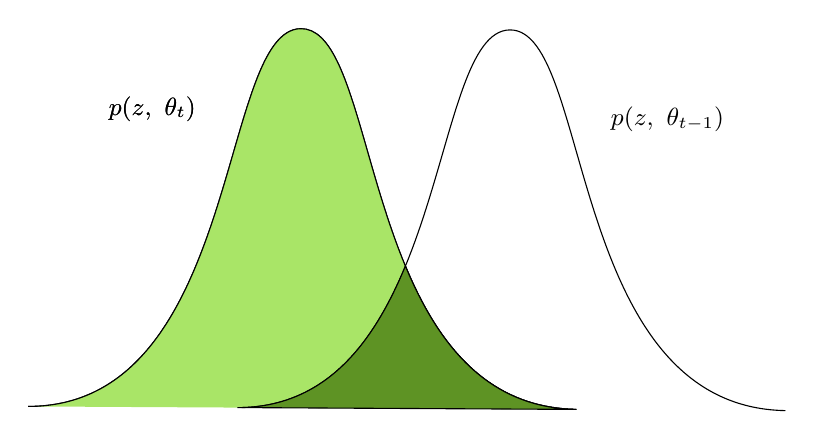
\begin{tikzpicture}[x=0.75pt,y=0.75pt,yscale=-1,xscale=1]
    %uncomment if require: \path (0,300); %set diagram left start at 0, and has height of 300
    
        \only<3>{
        %Shape: Boxed Bezier Curve [id:dp19284355666403086] 
        \draw    (163.42,256.57) .. controls (266.14,256.57) and (255.08,74.89) .. (294.76,74.57) .. controls (323.56,74.35) and (324.97,170.2) .. (363.9,223.42) .. controls (378.6,243.51) and (398.64,257.52) .. (427.52,258) ;
        \draw (201.02,105.96) node [anchor=north west][inner sep=0.75pt]  [font=\small]  {$p( z,\ \theta _{t})$};   
        }
        \onslide<4->{
        %Shape: Boxed Bezier Curve [id:dp19284355666403086] 
        \draw [fill={rgb, 255:red, 169; green, 229; blue, 103 }  ,fill opacity=1 ]   (163.42,256.57) .. controls (266.14,256.57) and (255.08,74.89) .. (294.76,74.57) .. controls (323.56,74.35) and (324.97,170.2) .. (363.9,223.42) .. controls (378.6,243.51) and (398.64,257.52) .. (427.52,258) ;
        \draw (201.02,105.96) node [anchor=north west][inner sep=0.75pt]  [font=\small]  {$p( z,\ \theta _{t})$};   
        }

        \onslide<2->{
        %Shape: Boxed Bezier Curve [id:dp5389195998778902] 
        \draw    (264.16,257.15) .. controls (366.88,257.15) and (355.82,75.47) .. (395.5,75.16) .. controls (435.18,74.84) and (422.87,256.84) .. (528.26,258.58) ;
        \draw (442.91,110.85) node [anchor=north west][inner sep=0.75pt]  [font=\small]  {$p( z,\ \theta _{t-1})$};
        }
        \onslide<4->{
        %Shape: Path Data [id:dp639977105939747] 
        \draw  [fill={rgb, 255:red, 94; green, 147; blue, 36 }  ,fill opacity=1 ] (363.9,223.42) .. controls (378.6,243.51) and (398.64,257.52) .. (427.52,258) -- (266.2,257.12) .. controls (307.63,256.14) and (330.18,225.11) .. (345.13,188.95) .. controls (350.31,201.36) and (356.41,213.18) .. (363.9,223.42) -- cycle ;
        }

    \end{tikzpicture}

    \end{figure}
\end{frame}


	% \include{slides/7-conclusion.tex}
	\begin{frame}{Content}
    \begin{enumerate}%
      \setlength\itemsep{1em}%
      \item {\color{lightgray} \ti{}} \tei{}
      \item {\color{lightgray} \tii{}} \teii{}
      \item {\color{lightgray} \tiii{}} \teiii{}
      \item {\color{lightgray} \tiv{}} \teiv{}
      \item {\color{lightgray} \tv{}} \tev{}
      \item {\color{lightgray} \tcvi{}} \tevi{}
    \end{enumerate}
  \end{frame}

% \begin{frame}{\tcvi{} Future work}
%     \onslide<2->{
%     \begin{block}{LUCI ES}
%         \begin{itemize}
%             \item Explore ($\mu , \lambda$) ES
%             \item Ranking in Bandit problems
%             \item Heritage (Importance Mixing, elitism)
%             \item Scalability
%         \end{itemize}
%     \end{block}
%     }
%     \onslide<3->{
%     \begin{block}{ES for Policy Search}
%         \begin{itemize}
%             \item Neuroevolution constraints and theory
%             % \item Theory of ES for policy search
%             \item Ablation study of existing methods
%         \end{itemize}
%     \end{block}
%     }
%     \onslide<4->{
%     \begin{block}{Evolving Evolution Strategies}
%         \begin{itemize}
%             \item Make ES methods emerge from scratch
%             % \item Improve current methods by bootstrapping from them
%             \item Neuromodulation: adapting ES during the evolution
%         \end{itemize}
%     \end{block}
%     }
    
% \end{frame}


\begin{frame}{\tcvi{} Future work}%
    \only<1>{
    \begin{block}{LUCI ES}
        \begin{itemize}
            \item Explore ($\mu , \lambda$) ES
            \item Ranking in Bandit problems
            \item Heritage (Importance Mixing, elitism)
            \item Scalability
        \end{itemize}
    \end{block}
    }
    \only<2>{
    \begin{block}{Evolving Evolution Strategies}
        \begin{itemize}
            \item Make ES methods emerge from scratch
            % \item Improve current methods by bootstrapping from them
            \item Neuromodulation: adapting ES during the evolution
        \end{itemize}
    \end{block}
    }
    \only<3>{
    \begin{block}{ES for Policy Search}
        \begin{itemize}
            \item Neuroevolution constraints and theory
            % \item Theory of ES for policy search
            \item Ablation study of existing methods
        \end{itemize}
    \end{block}
    }
    \only<4>{
    }
    \begin{figure}
        \tikzset{every picture/.style={line width=0.75pt}} %set default line width to 0.75pt        

        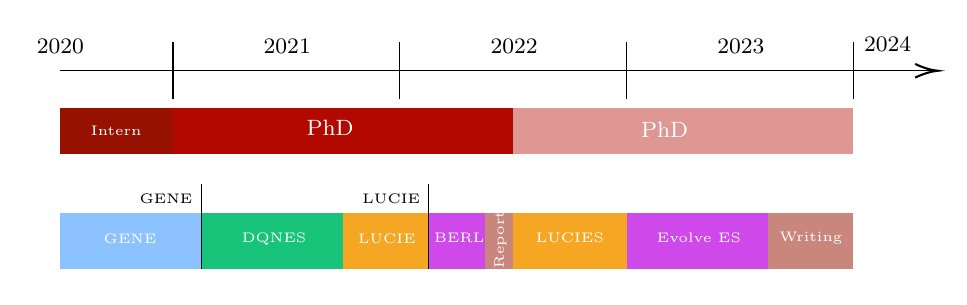
\begin{tikzpicture}[x=0.75pt,y=0.75pt,yscale=-1,xscale=1]
        %uncomment if require: \path (0,300); %set diagram left start at 0, and has height of 300
        
        
        %Straight Lines [id:da263455807473124] 
        \draw    (145.56,104.38) -- (566.71,104.38) ;
        \draw [shift={(568.71,104.38)}, rotate = 180] [color={rgb, 255:red, 0; green, 0; blue, 0 }  ][line width=0.75]    (10.93,-3.29) .. controls (6.95,-1.4) and (3.31,-0.3) .. (0,0) .. controls (3.31,0.3) and (6.95,1.4) .. (10.93,3.29)   ;
        %Straight Lines [id:da06908695747928117] 
        \draw    (200.2,90.72) -- (200.2,118.04) ;
        %Straight Lines [id:da3172970011493099] 
        \draw    (309.48,90.72) -- (309.48,118.04) ;
        %Straight Lines [id:da7182015191619326] 
        \draw    (418.76,90.72) -- (418.76,118.04) ;
        %Straight Lines [id:da5499230746738971] 
        \draw    (528.04,90.72) -- (528.04,118.04) ;
        %Shape: Rectangle [id:dp3072423219363737] 
        \draw  [draw opacity=0][fill={rgb, 255:red, 179; green, 8; blue, 0 }  ,fill opacity=1 ] (200.2,122.14) -- (364.12,122.14) -- (364.12,144.69) -- (200.2,144.69) -- cycle ;
        %Shape: Rectangle [id:dp48101964277359865] 
        \draw  [draw opacity=0][fill={rgb, 255:red, 179; green, 8; blue, 0 }  ,fill opacity=0.42 ] (364.12,122.14) -- (528.04,122.14) -- (528.04,144.69) -- (364.12,144.69) -- cycle ;
        %Shape: Rectangle [id:dp8094283759581382] 
        \draw  [draw opacity=0][fill={rgb, 255:red, 150; green, 17; blue, 0 }  ,fill opacity=1 ] (145.56,122.14) -- (200.2,122.14) -- (200.2,144.69) -- (145.56,144.69) -- cycle ;
        %Shape: Rectangle [id:dp25218225952021045] 
        \draw  [draw opacity=0][fill={rgb, 255:red, 140; green, 194; blue, 255 }  ,fill opacity=1 ] (145.56,172.68) -- (213.86,172.68) -- (213.86,200) -- (145.56,200) -- cycle ;
        %Shape: Rectangle [id:dp439106993654921] 
        \draw  [draw opacity=0][fill={rgb, 255:red, 24; green, 195; blue, 122 }  ,fill opacity=1 ] (213.86,172.68) -- (282.16,172.68) -- (282.16,200) -- (213.86,200) -- cycle ;
        %Shape: Rectangle [id:dp07333800236304988] 
        \draw  [draw opacity=0][fill={rgb, 255:red, 245; green, 166; blue, 35 }  ,fill opacity=1 ] (282.16,172.68) -- (323.14,172.68) -- (323.14,200) -- (282.16,200) -- cycle ;
        %Shape: Rectangle [id:dp055858616927162985] 
        \draw  [draw opacity=0][fill={rgb, 255:red, 150; green, 17; blue, 0 }  ,fill opacity=0.51 ] (350.46,172.68) -- (364.12,172.68) -- (364.12,200) -- (350.46,200) -- cycle ;
        %Shape: Rectangle [id:dp7612465684991917] 
        \draw  [draw opacity=0][fill={rgb, 255:red, 245; green, 166; blue, 35 }  ,fill opacity=1 ] (364.12,172.68) -- (418.76,172.68) -- (418.76,200) -- (364.12,200) -- cycle ;
        %Shape: Rectangle [id:dp6656802192707113] 
        \draw  [draw opacity=0][fill={rgb, 255:red, 207; green, 72; blue, 234 }  ,fill opacity=1 ] (323.14,172.68) -- (350.46,172.68) -- (350.46,200) -- (323.14,200) -- cycle ;
        %Shape: Rectangle [id:dp8472926104883064] 
        \draw  [draw opacity=0][fill={rgb, 255:red, 150; green, 17; blue, 0 }  ,fill opacity=0.51 ] (487.06,172.68) -- (528.04,172.68) -- (528.04,200) -- (487.06,200) -- cycle ;
        %Shape: Rectangle [id:dp6374386242575871] 
        \draw  [draw opacity=0][fill={rgb, 255:red, 207; green, 72; blue, 234 }  ,fill opacity=1 ] (418.76,172.68) -- (487.06,172.68) -- (487.06,200) -- (418.76,200) -- cycle ;
        %Straight Lines [id:da43034538559618607] 
        \draw    (213.86,159.02) -- (213.86,200) ;
        %Straight Lines [id:da5380962385035739] 
        \draw    (323.14,159.02) -- (323.14,200) ;
        %Straight Lines [id:da3604388553748691] 
        % \draw    (418.76,159.02) -- (418.76,200) ;
        
        % Text Node
        \draw (364.53,92.77) node  [font=\footnotesize] [align=left] {2022};
        % Text Node
        \draw (255.25,92.77) node  [font=\footnotesize] [align=left] {2021};
        % Text Node
        \draw (145.97,92.77) node  [font=\footnotesize] [align=left] {2020};
        % Text Node
        \draw (473.81,92.77) node  [font=\footnotesize] [align=left] {2023};
        % Text Node
        \draw (544.5,91.5) node  [font=\footnotesize] [align=left] {2024};
        % Text Node
        \draw (179.54,185.45) node  [font=\tiny,color={rgb, 255:red, 255; green, 255; blue, 255 }  ,opacity=1 ] [align=left] {GENE};
        % Text Node
        \draw (248.92,185.45) node  [font=\tiny,color={rgb, 255:red, 255; green, 255; blue, 255 }  ,opacity=1 ] [align=left] {DQNES};
        % Text Node
        \draw (303.28,185.45) node  [font=\tiny,color={rgb, 255:red, 255; green, 255; blue, 255 }  ,opacity=1 ] [align=left] {LUCIE};
        % Text Node
        \draw (357.97,185.66) node  [font=\fontsize{0.33em}{0.4em}\selectfont,color={rgb, 255:red, 255; green, 255; blue, 255 }  ,opacity=1 ,rotate=-270] [align=left] {Report};
        % Text Node
        \draw (391.44,184.97) node  [font=\tiny,color={rgb, 255:red, 255; green, 255; blue, 255 }  ,opacity=1 ] [align=left] {LUCIES};
        % Text Node
        \draw (338.17,184.97) node  [font=\tiny,color={rgb, 255:red, 255; green, 255; blue, 255 }  ,opacity=1 ] [align=left] {BERL};
        % Text Node
        \draw (507.55,184.97) node  [font=\tiny,color={rgb, 255:red, 255; green, 255; blue, 255 }  ,opacity=1 ] [align=left] {Writing};
        % Text Node
        \draw (453.59,184.97) node  [font=\tiny,color={rgb, 255:red, 255; green, 255; blue, 255 }  ,opacity=1 ] [align=left] {Evolve ES};
        % Text Node
        \draw (196.79,165.85) node  [font=\tiny] [align=left] {GENE};
        % Text Node
        \draw (305.38,165.85) node  [font=\tiny] [align=left] {LUCIE};
        % Text Node
        % \draw (397.59,165.85) node  [font=\tiny] [align=left] {LUCIES};
        % Text Node
        \draw (279.43,131.81) node  [font=\footnotesize,color={rgb, 255:red, 255; green, 255; blue, 255 }  ,opacity=1 ] [align=left] {\begin{minipage}[lt]{22.29pt}\setlength\topsep{0pt}
        PhD
        \end{minipage}};
        % Text Node
        \draw (440.62,132.81) node  [font=\footnotesize,color={rgb, 255:red, 255; green, 255; blue, 255 }  ,opacity=1 ] [align=left] {\begin{minipage}[lt]{22.29pt}\setlength\topsep{0pt}
        PhD
        \end{minipage}};
        % Text Node
        \draw (174.25,133.26) node  [font=\tiny,color={rgb, 255:red, 255; green, 255; blue, 255 }  ,opacity=1 ] [align=left] {\begin{minipage}[lt]{20.36pt}\setlength\topsep{0pt}
        Intern
        \end{minipage}};
        
        \end{tikzpicture}

    \end{figure}
\end{frame}
	
	\newcounter{lastframe}
	\setcounter{lastframe}{\insertframenumber}
	
	\begin{frame}[allowframebreaks]{References}
		% \bibliographystyle{authoryear-fr}
		% \bibliographystyle{abbrv}
		\bibliographystyle{apalike}
		\bibliography{references}
	\end{frame}

	


% Bounded identity
\begin{frame}{\tciii{} Signed distances}

\begin{columns}
\begin{column}{0.45\linewidth}
\begin{block}{Bounded identity function}
\begin{equation}
\alpha: \begin{cases}
& \text{ if } x \geq 1: \alpha(x) = 1\\ 
& \text{ if } x \leq -1: \alpha(x) = -1\\ 
& \text{ else: }  \alpha(x) = x
\end{cases}
\end{equation}
\end{block}
\end{column}

\begin{column}{0.45\linewidth}
\begin{figure}
\centering
\includegraphics[width=.9\linewidth]{images/GENE/images/bounded.png}
\end{figure}
\end{column}
\end{columns}

\end{frame}


% Final functions
\begin{frame}{\tciii{} Distance functions}

\begin{columns}
\begin{column}{0.60\linewidth}
\begin{block}{pL2-GENE}
\begin{equation}
\alpha \left  ( \prod_{k=1}^D n_1^k - n_2^k \right ) \sqrt{\sum_{j=1}^D \left( n_1^j - n_2^j \right)^2 }
\end{equation}
\end{block}
\end{column}

\begin{column}{0.35\linewidth}
\begin{figure}
\centering
\includegraphics[width=\linewidth]{images/GENE/images/distance_pL2.png}
\end{figure}
\end{column}
\end{columns}

\begin{columns}
\begin{column}{0.60\linewidth}
\begin{block}{tag-GENE}
\begin{equation}
\sum_{j=2}^D \alpha(n_1^j - n_2^1) e^{-|n_1^j - n_2^1|}
\end{equation}
\end{block}
\end{column}

\begin{column}{0.35\linewidth}
\begin{figure}
\centering
\includegraphics[width=\linewidth]{images/GENE/images/distance_tag.png}
\end{figure}
\end{column}
\end{columns}

\end{frame}


\begin{frame}{\tcv{} Classic Control}%
        \def\figwidth{0.16\linewidth}%
        \def\yleg{Fitness}%
        \begin{textblock*}{2cm}(0cm,0.7cm) % {block width} (coords)
            $\%$noise
        \end{textblock*}
        \begin{table}%[!t]
            \centering
            \begin{tabular}{ccccccc}
                && $0\%$ & $200\%$ & $400\%$ & $600\%$ & $800\%$ \\
                \raisebox{3\normalbaselineskip}[0pt][0pt]{\rotatebox[origin=c]{90}{\cartpole}} &
                \raisebox{3\normalbaselineskip}[1cm][0cm]{\rotatebox[origin=c]{90}{\vspace{1cm}\yleg}}&
                \includegraphics[width=\figwidth]{images/LUCIE/cartpole/boxplot_cartpole_0.png} &
                \includegraphics[width=\figwidth]{images/LUCIE/cartpole/boxplot_cartpole_200.png} &
                \includegraphics[width=\figwidth]{images/LUCIE/cartpole/boxplot_cartpole_400.png} &
                \includegraphics[width=\figwidth]{images/LUCIE/cartpole/boxplot_cartpole_600.png} &
                \includegraphics[width=\figwidth]{images/LUCIE/cartpole/boxplot_cartpole_800.png}\\
            \end{tabular}
%				\caption{Final validation fitness for \cartpole{} neuroevolution under posterior uniform noise.}
%				\label{table:cartpole-uniform-eval-validation}
        \end{table}

        \vspace{-1em}

        \def\figwidth{0.16\linewidth}
        \def\yleg{Fitness}
        \begin{table}[]
            \centering
            \begin{tabular}{ccccccc}
%					&& 0\% & 200\% & 400\% & 600\% & 800\% \\
                \raisebox{3.5\normalbaselineskip}[0pt][0pt]{\rotatebox[origin=c]{90}{\acrobot{}}} &
                \raisebox{3.5\normalbaselineskip}[1cm][0cm]{\rotatebox[origin=c]{90}{\vspace{1cm}\yleg}}&
                \includegraphics[width=\figwidth]{images/LUCIE/acrobot/boxplot_acrobot_0_u.png} &
                \includegraphics[width=\figwidth]{images/LUCIE/acrobot/boxplot_acrobot_200_u.png} &
                \includegraphics[width=\figwidth]{images/LUCIE/acrobot/boxplot_acrobot_400_u.png} &
                \includegraphics[width=\figwidth]{images/LUCIE/acrobot/boxplot_acrobot_600_u.png} &
                \includegraphics[width=\figwidth]{images/LUCIE/acrobot/boxplot_acrobot_800_u.png}\\
            \end{tabular}
%				\caption{Final validation fitness for Acrobot neuroevolution under posterior uniform noise.}
%				\label{table:acrobot-uniform-eval-validation}
        \end{table}

\end{frame}
	
	\setcounter{framenumber}{\thelastframe}

\end{document}
